\documentclass[11pt,a4paper]{article}
\usepackage[margin=24mm]{geometry}\usepackage{fontspec,unicode-math,booktabs,graphicx,hyperref}
\setmainfont{STIXGeneral}\setmathfont{STIX Two Math}
\title{Rank augmentation:\\complete manuscript and program costs}
\author{Human Compression project}\date{}
\begin{document}\maketitle
The original is De Saedeleer--Leemans--Mulpas, \emph{A rank augmentation
theorem for rank 3 string C-group representations of the symmetric groups},
arXiv:2212.12563v1, 23 December 2022 (L020). All nineteen pages are counted,
including the banner, introductory table, diagrams, references and addresses.
The nineteen accepted dispositions preserve the valid first two cases of
Theorem~4.1 and replace its false third case by an exact criterion and a
complete eighteen-point counterexample. The original retains its literal
claims in every measured representation. This is one original, not two.

\paragraph{The complete written comparison.}
For raw, untrimmed extraction in NFC, counting characters without whitespace,
\[
R_{\rm written}=\frac{33604}{13904+(7242+6854)}
=\frac{33604}{28000}=1.200143.
\]
The whole five-page common paper and both three-page local papers are paid.
The counterproof is a required application dependency; citing an earlier
correction does not make it free. No old Topic B common theory or cross-topic
saving is assumed. Titles, references and repeated exposition remain charged.
\begin{center}\begin{tabular}{lrr}\toprule
Complete document&Pages&Characters\\\midrule
Original L020&19&33604\\
Common supported-transposition proof&5&13904\\
Source application&3&7242\\
Required counterexample proof&3&6854\\
All three programs, printed&3&10866\\\bottomrule
\end{tabular}\end{center}
\paragraph{Complete programs and the conditional application.}
Including the whole program appendix gives the separate comparison
$33604/(28000+10866)=0.864612$.
The three whole raw programs cost 9998 characters and give
$33604/(28000+9998)=0.884362$. Printed and raw programs are alternatives;
the old two-page appendix is replaced, not added.
The program-inclusive denominators exceed the source length in this coordinate.

After acquiring \emph{the entire common paper, all three declared programs
and all retained premises}, the complete six-page local application costs
14096 characters:
\[
r\mid(U,\mathrm{programs})=33604/(7242+6854)=2.383939.
\]
This is a conditional acquisition comparison, not the whole-topic factor.
The source-example program supplies finite certificates; the model program
is bounded validation; the eighteen-point certificate supports the complete
written counterproof. No bounded test replaces a uniform proof.

\paragraph{Separate and unknown costs.}
Three drivers cost 14096 nonspace characters (15,947 literal bytes).
Two whole Lean files cost 5218 characters (6,855 bytes), with two generic
and thirteen literal-obstruction declarations, not a full source formalization.
The motivating Table~1 census and classical end criterion remain retained;
full outside-proof, runtime, historical-software, graphic and formalization
costs are unknown, not zero. These are complete-text representation lengths,
not minimum proof complexity or research effort. No new scientific credit is
assigned by this numerical packet.
\newpage
\begin{center}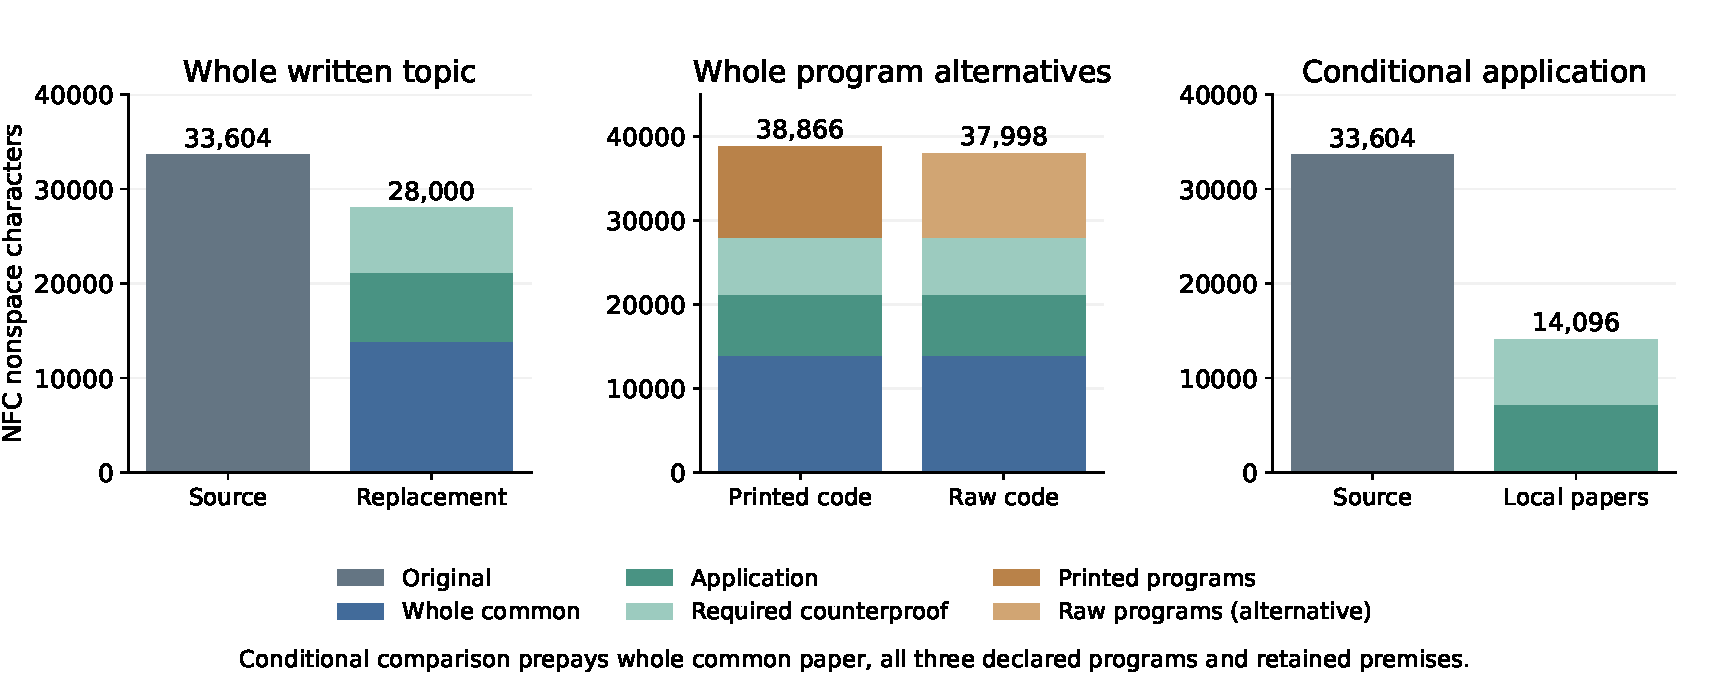
\includegraphics[width=\textwidth]{costs.pdf}\end{center}
\vspace{-4mm}
\begin{center}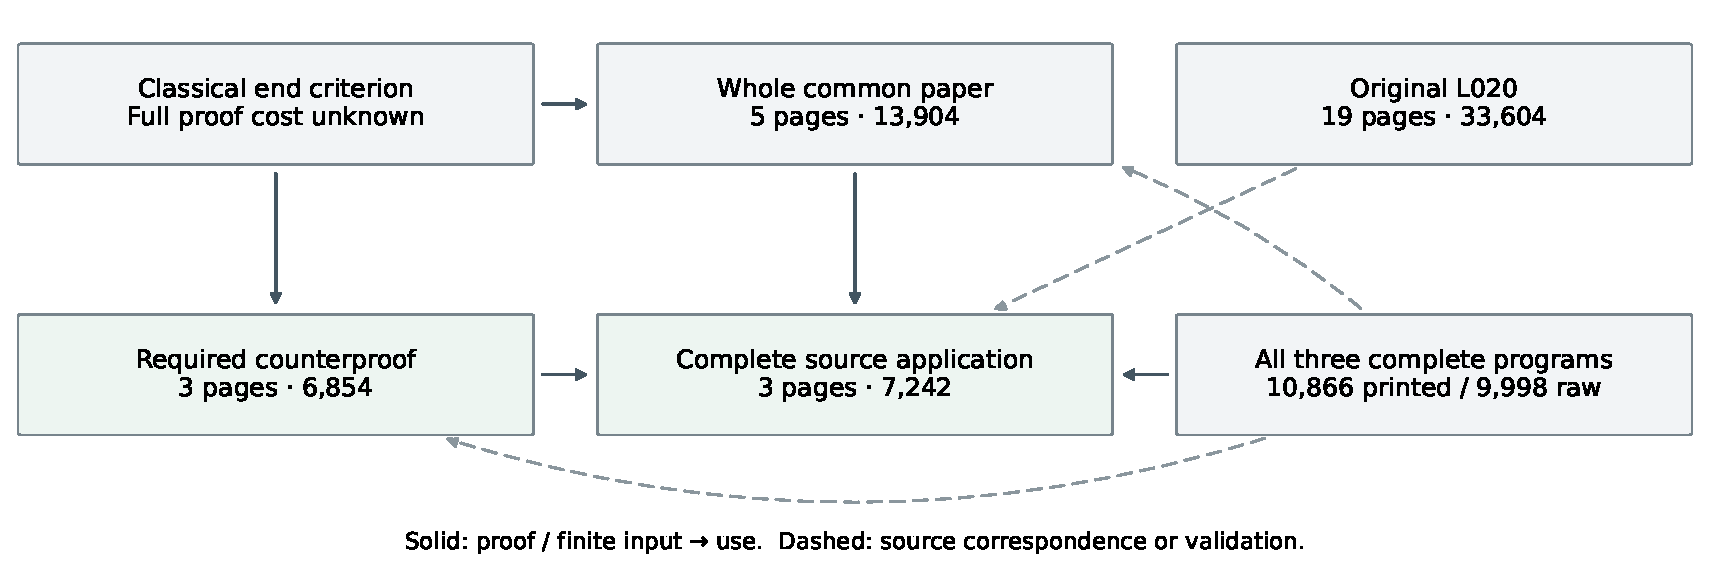
\includegraphics[width=\textwidth]{document_graph.pdf}\end{center}
\vspace{-4mm}
The graph distinguishes proof dependencies from source correspondence and
validation. It does not remove any document from the cost. In particular,
the counterproof stays in the local application and the common paper is
charged once. Whole-document acquisition sums and every raw file are also
available in JSON/CSV; no node-count factor is used.

\paragraph{Unit and encoding sensitivities.}
Raw, untrimmed NFC coordinates are:
\begin{center}\small\begin{tabular}{lrrrr}\toprule
Unit&Written&Printed&Raw&Conditional\\\midrule
Whitespace tokens & 1.365 & 1.202 & 1.226 & 2.817 \\
Alphanumeric units & 1.385 & 1.010 & 1.028 & 2.812 \\
Nonspace characters & 1.200 & 0.865 & 0.884 & 2.384 \\
Collapsed-space characters & 1.231 & 0.917 & 0.938 & 2.462 \\
Collapsed-space UTF-8 bytes & 1.158 & 0.886 & 0.904 & 2.361 \\
\bottomrule\end{tabular}\end{center}
All thirty coordinates and 120 exact fractions are retained: five units,
NFC and NFKC, with untrimmed, furniture-selected and calibrated-selected
text. Selection removes only exact repeated headers and isolated page
numbers. Two actual font/byte classes account for 112 observed substitutions:
111 calligraphic G symbols and one blackboard-bold N. The raw coordinates
are unchanged. The arXiv banner remains included; printed hyphens remain
literal. Full diagram topology, colour, curvature and layout are not
reconstructed from extracted labels, so graphic complexity stays unknown.
Normalized text-byte units differ from literal stored-file bytes.

\paragraph{Review boundary.}
Scientific acceptance and the distinct input review are reused. The numerical
author previously reviewed those inputs but did not author them; this new
arithmetic and reader require a distinct numerical review. The source's
larger-orbit and higher-rank questions remain unresolved. No source, question
or formal credit is added here.
\end{document}
